\documentclass{beamer}


\usepackage[utf8]{inputenc}
\usepackage[T1]{fontenc}
\usepackage[english]{babel}
\usepackage{color}
\usepackage{graphicx} % Allows including images
\usepackage{booktabs} % Allows the use of \toprule, \midrule and \bottomrule in tables
\usepackage{amsmath}
\usepackage{amssymb}
\usepackage{overpic}
\usepackage[font=footnotesize, caption=true]{subfig}
\usepackage{multirow}
\usepackage{tikz}
\usepackage{enumitem}
\usepackage{tikz}
\usetikzlibrary{shapes.geometric, arrows}
\usepackage{textpos}
\usepackage{multimedia}
\usepackage[framemethod=tikz]{mdframed}
\usepackage{xcolor}

\usepackage{fontawesome} 
\usepackage[lf]{venturis} 


\newcommand{\imagepath}{Images}

\mode<presentation>
{
\usetheme{default}
}

\makeatletter
\@addtoreset{subfigure}{framenumber}% subfigure counter resets every frame
\makeatother

\makeatletter
\definecolor{beamer@blendedblue}{rgb}{0.2,0.4.0,0.2} % changed this

\setbeamercolor{normal text}{fg=black,bg=white}
\setbeamercolor{alerted text}{fg=red}
\setbeamercolor{example text}{fg=green!50!black}

\setbeamercolor{structure}{fg=beamer@blendedblue}

\setbeamercolor{background canvas}{parent=normal text}
\setbeamercolor{background}{parent=background canvas}

\setbeamercolor{palette primary}{fg=yellow,bg=yellow} % changed this
\setbeamercolor{palette secondary}{use=structure,fg=structure.fg!100!green} % changed this
\setbeamercolor{palette tertiary}{use=structure,fg=structure.fg!100!green} % changed this
\makeatother

\newmdenv[tikzsetting={draw=black,fill=white,fill opacity=0.7, line width=4pt},backgroundcolor=none,leftmargin=0,rightmargin=0,innertopmargin=4pt,skipbelow=\baselineskip,%
skipabove=\baselineskip]{TitleBox}

 
\title[] % (optional, use only with long paper titles)
{MWE for video in beamer}

\author[Tabb, Tabb]
{
  Amy~Tabb
}

\date{\today} % Date, can be changed to a custom date



%----------------------------------------------------------------------------------------
\begin{document}

% Fancy title page, using transparent text box from mdframe, and icon from fontawesome
{  \usebackgroundtemplate{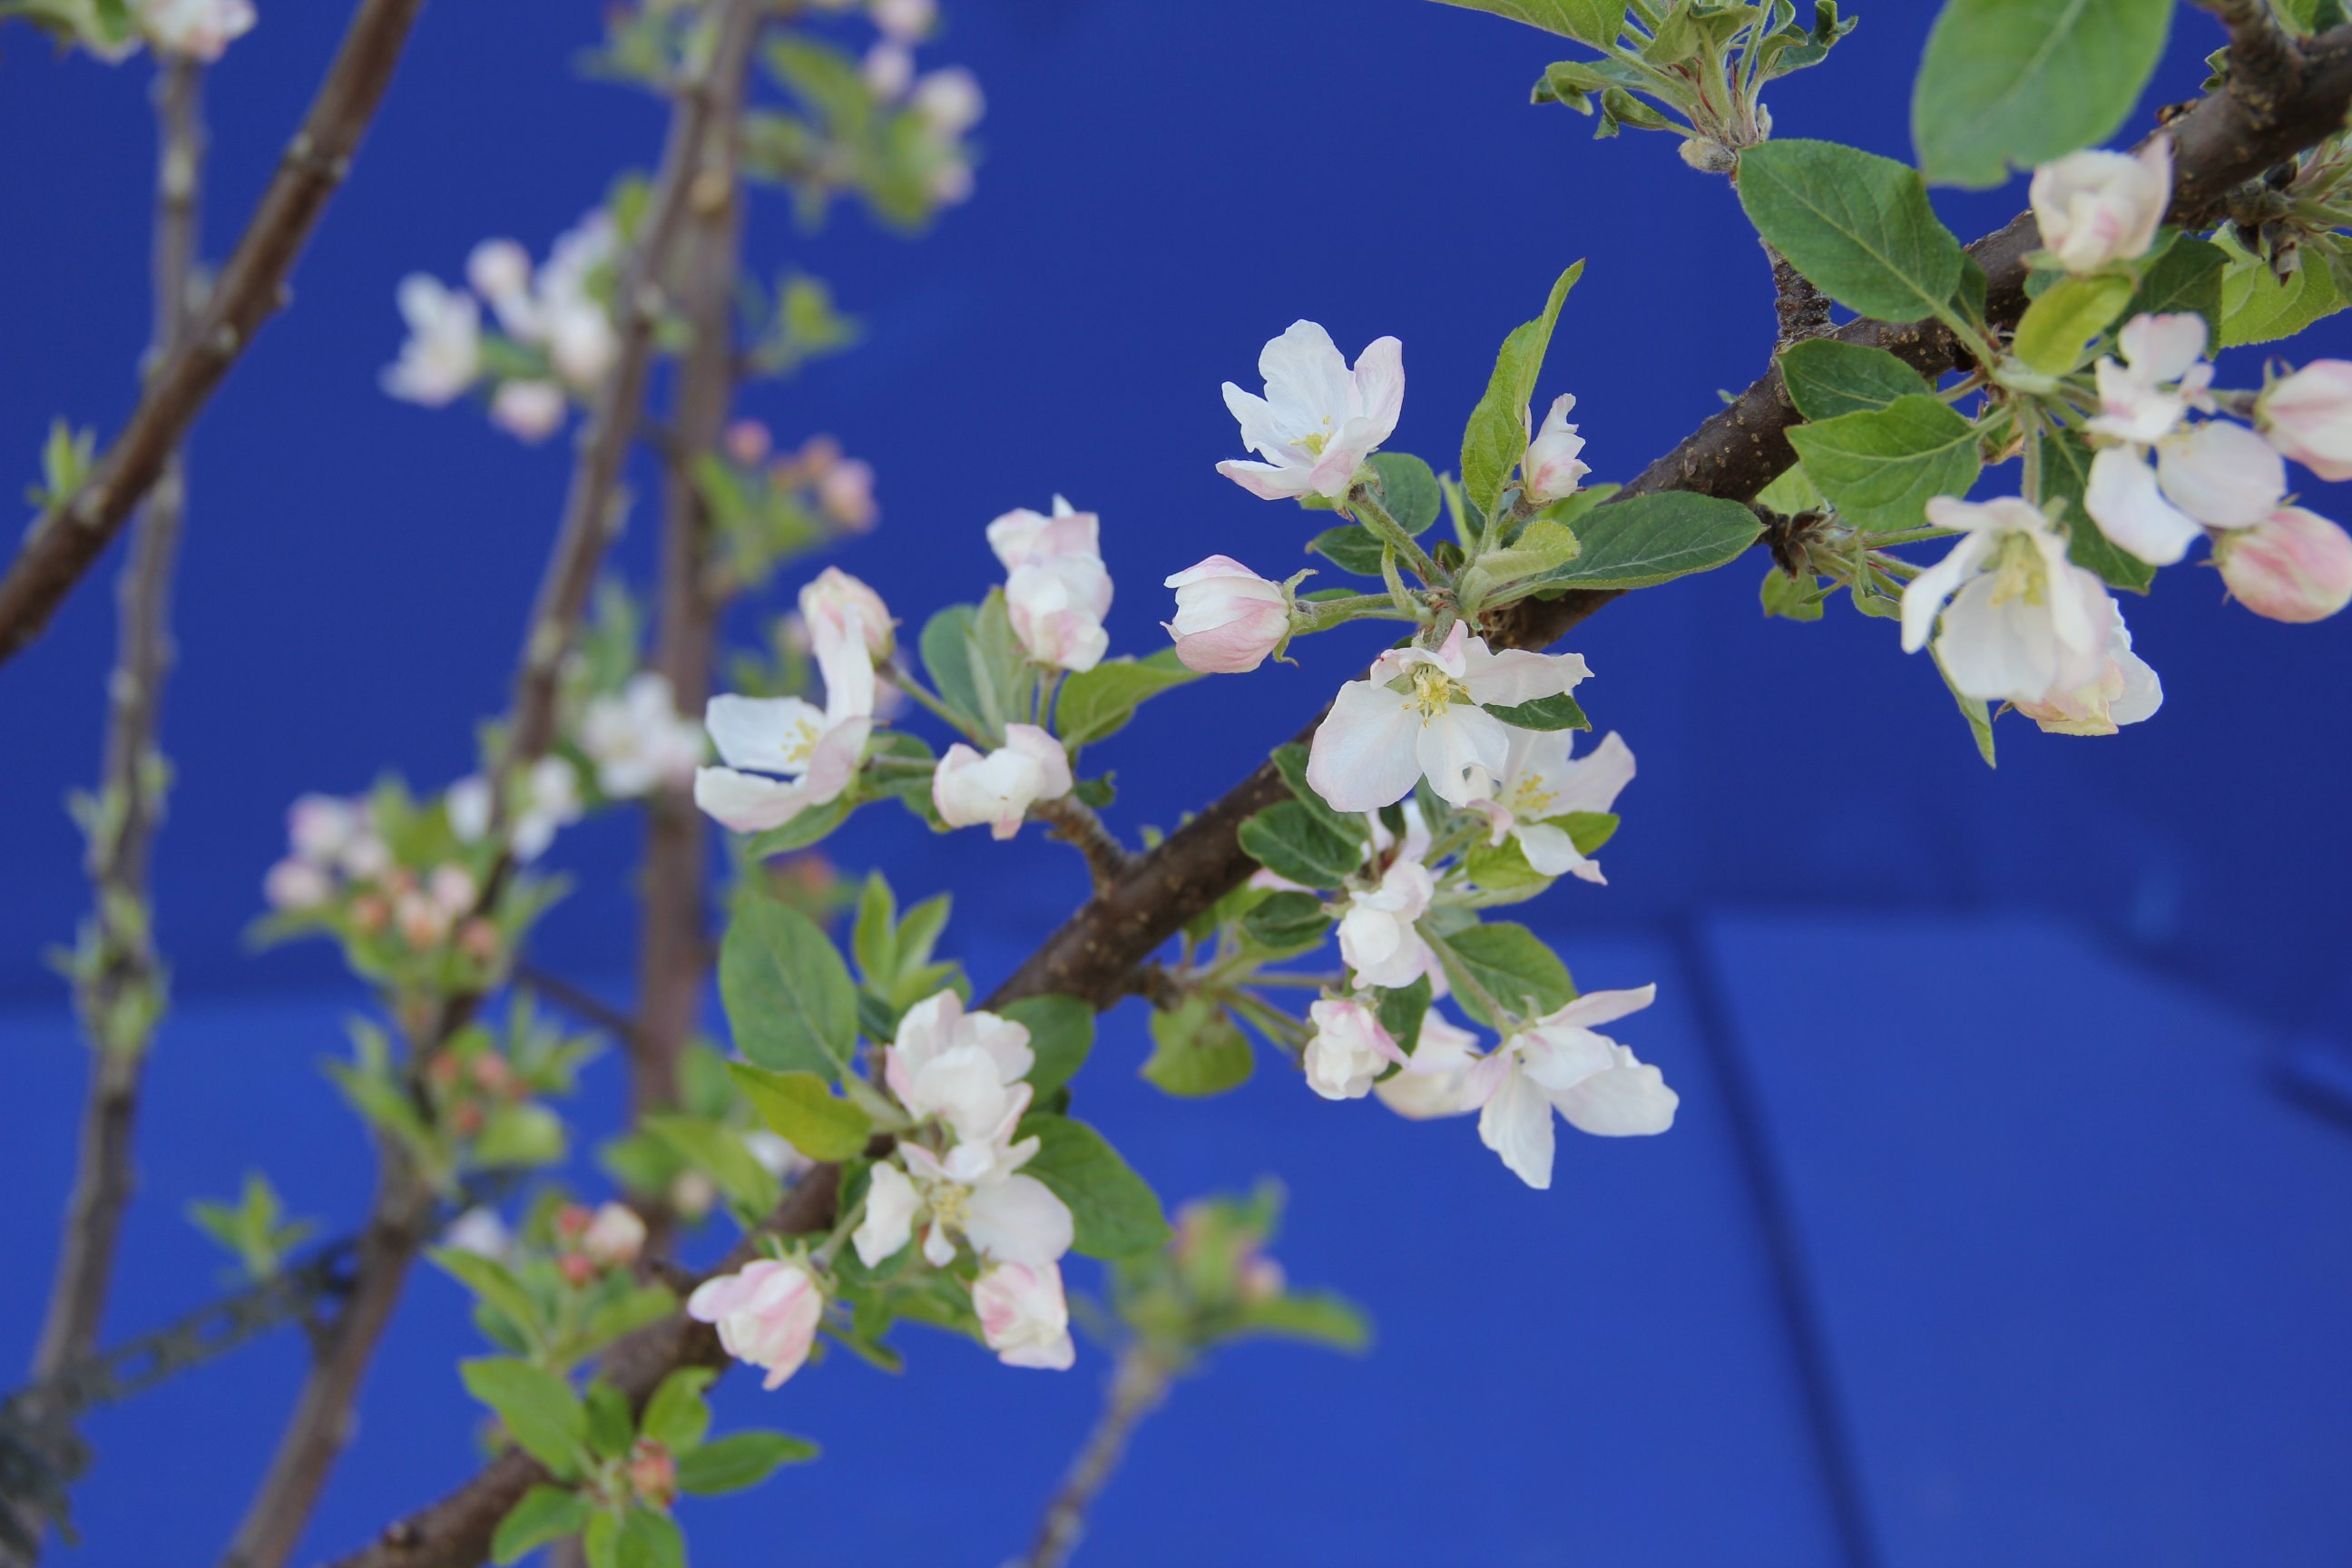
\includegraphics[width=1.0\paperwidth]{\imagepath/IMG_1373-resize.jpg}}
  \begin{frame}[plain] 

  \vspace{15em}

  \begin{TitleBox}
 
{\large MWE for video in beamer }
    
    Amy Tabb\\
    \faTwitter @amy\_tabb
   
   
   \end{TitleBox}

  \end{frame}
}


%%%%%%%%%%%%%% VIDEO  %%%%%%%%%%%%%%%%%%%%%%%%%%%%%%%%%%
\begin{frame}
\frametitle{Test video} 

\center
\movie[label=show3, height = 6cm, poster, autostart, showcontrols]{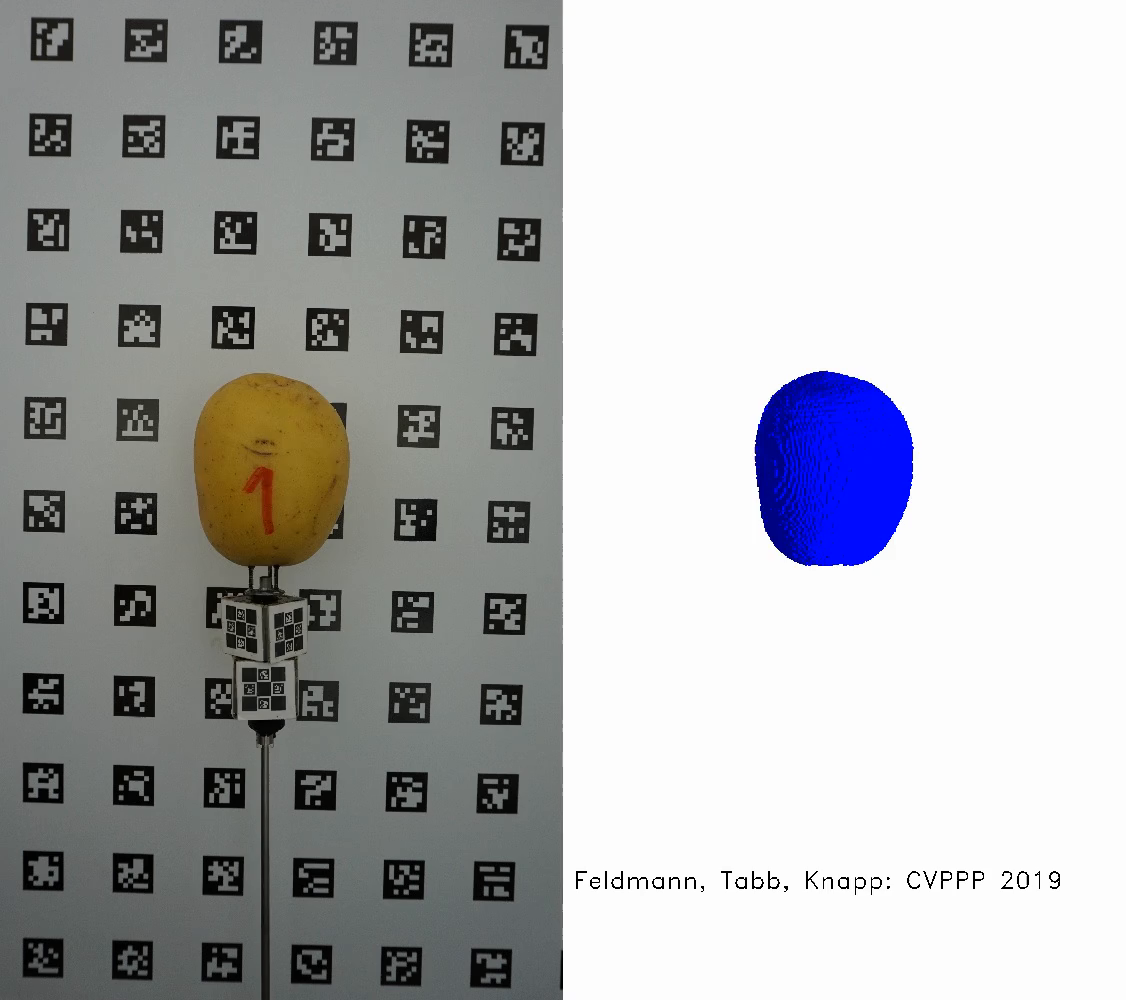
\includegraphics[height = 6cm]{\imagepath/Potato-poster.png}}{\imagepath/Potato.mp4}

\end{frame}

\end{document}
